\chapter{\vnnlib{} Query Language}\label{sec:specification_language}

At the heart of the \vnnlib{} standard is the \vnnlib{} query language. Heavily influenced by SMT-LIB, this language is designed as a standardised computer-readable format for expressing a wide range of satisfiability problems over neural networks. This chapter describes the syntax, scoping, typing and semantics of the query language.

\section{Syntax}
\label{sec:syntax}


Similar to SMT-LIB, the syntax of \vnnlib{} is primarily designed with the goal of machine-readability in mind. Although the syntax is somewhat human-readable, maximising readability is not a primary goal of the language. Instead it is envisaged that \vnnlib{} queries will be generated automatically by higher level tools that provide better user-orientated interfaces.

The syntax of \vnnlib{} is formally defined as Labelled Backus-Naur Form~\cite{8} (LBNF) grammar which can be found in Appendix~\ref{app:lbnf_grammar}. Instead of describing each of the production rules in detail, we will now highlight key syntactic constructs of the language via examples illustrating their usage.

Firstly, all \vnnlib{} queries are split into two parts: a list of network declarations and a list of assertions. The former allow users to specify an interface for the networks and bring new abstract variables into scope that represent the input and output values of the network. The latter than reference those variables in order to express the desired constraints that should be satisfied. Currently, the standard does not permit the interleaving of network declarations and assertions. Figure~\ref{fig:simple-query} shows an example of a simple query.

\subsection{Simple network declarations}
\label{sec:network-declarations}

 At its simplest, a network is introduced by the keyword \texttt{declare-network}, followed by a user-defined name for the network, and then declarations for its associated input and output. An input is declared using the \texttt{declare-input} keyword, followed by a variable name, its element type (e.g., \texttt{Real}, \texttt{float64}), 
and the shape of the tensor. Similarly, an output variable uses the \texttt{declare-output} keyword. In the case of Figure~\ref{fig:simple-query}, the network is named \texttt{myNetwork}, and it has one input called \texttt{X} consisting of a $1 \times 10$ tensor of real numbers and one output called \texttt{Y} consisting of a $1 \times 2$ tensor of real numbers. 
\begin{figure}[t]
    \begin{minipage}[c]{0.6\textwidth}
        \begin{lstlisting}[style=lbnf]
(declare-network myNetwork
    (declare-input  X Real [1,10])
    (declare-output Y Real [1,2])
)

(assert (>= X[0,2] 0.0))
(assert (<= X[0,2] 1.0))
(assert (<= Y[0,1] 0.5))\end{lstlisting}
    \end{minipage}%
    \begin{minipage}[c]{0.45\textwidth}
        \centering
        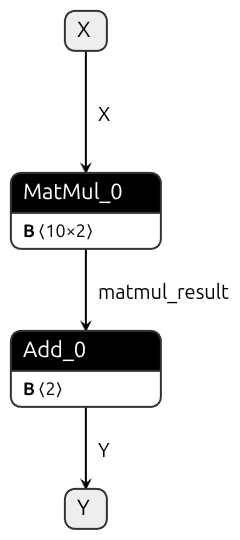
\includegraphics[height=5cm]{imgs/simple_net.onnx.png}
    \end{minipage}
    \caption{A simple \vnnlib{} specification which declares a network with a single input and output. An example of one of the many possible ONNX models compatible with this declaration is shown on the right. Note that the variable names in the declared inputs and outputs do not have to match the node names in the ONNX file.}
    \label{fig:simple-query}
\end{figure}


It is important to clarify that a network declaration only declares an \emph{interface} and by default does not refer in any way to a particular ONNX network model. When passing a query and a network to the verifier, the name of the network does not need to match the name of the ONNX model file. Instead, as described in Section~\ref{sec:verify_command}, the user will explicitly associate a network declaration to the relevant model file via the command line.
Neither do the declared names of the inputs and outputs need to match the names of the input and output nodes within the model file. This flexibility allows many different alternative ONNX models to be compatible with the same query.

All variable names follow the same syntax conventions: they are case-sensitive, must start with a letter, and may only contain letters, digits and underscores. All variable names must be unique within the query (see Section~\ref{sec:scoping} for a more in-depth discussion). 


% The \texttt{@} character is a reserved character which is used to denote multiple applications of the same network, for the purpose of defining  hyperproperties such as monotonicity. For example \texttt{(declare-network acasXu@1 ...)} and \texttt{(declare-network acasXu@2 ...)} define two networks that are both instances of the same ONNX model,  denoted as \texttt{acasXu} in the command line interface of the verifier (See Chapter~\ref{sec:solver_interface} for more details).

\subsection{Assertions}

The second part of a \vnnlib{} query is a list of assertions that constrain the abstract tensor variables introduced by the network declarations. \vnnlib{} supports quantifier-free logical formulas as \textit{assertions}. Assertions are defined using parenthesized \texttt{(assert\ldots)} expressions, and following an SMT-LIB-like prefix syntax with the 
operator preceding its operands. An assertion is a logical formula that may include logical connectives, relational comparisons, and arithmetic expressions over declared tensors and constants.
The final satisfiability problem is then the conjunction of all the assertions.
 
\paragraph{Constants}

Numeric constant values may be referenced using basic standard integer or floating point syntax (e.g. \inlinevnn{0}, \inlinevnn{0.0}, \inlinevnn{-0.5}). 

\paragraph{Variables} 

Standard indexing notation may be used to refer to a specific element within the tensor variable. For example, Line 6 in Figure~\ref{fig:simple-query} uses \inlinevnn{X[0,2]}, to refer to the value of the element of the input tensor at row~0, column~2. All indices are zero based and currently the number of indices provided must be equal to the number of dimensions of the variable, i.e. partial indexing is not allowed.

\paragraph{Arithmetic expressions}

One forms arithmetic expressions by recursively combining constant and variable values via prefix notation. Currently the following operators are supported:
\begin{itemize}
	\item \inlinevnn{(- a)}: Negation of a term.
    \item \inlinevnn{(+ a b ...)}: Addition of two or more terms. 
    \item \inlinevnn{(* a b ...)}: Multiplication of two or more terms. 
    \item \inlinevnn{(- a b ...)}: Subtraction of two or more terms. Note that subtraction associates to the left, e.g. \inlinevnn{(- 1 2 3 4)} is the same as \inlinevnn{(- (- (- 1 2) 3) 4)} .
\end{itemize}
Arithmetic operations currently only operate over individual tensor elements and cannot be used to operate over multi-dimensional tensors (see Section~\ref{sec:scoping_and_typing} for detailed typing rules).

\paragraph{Comparisons}

The comparison operators \inlinevnn{<=}, \inlinevnn{>=}, \inlinevnn{<}, \inlinevnn{>}, \inlinevnn{=}, \inlinevnn{!=} can be used to compare the values of two arithmetic operations.
For example, \inlinevnn{(<= a b)} returns true if $a$ is less than or equal to $b$.
    
\paragraph{Boolean expressions} 

One forms boolean expressions by recursively combining comparisons via the following supported logical connectives:
\begin{itemize}
    \item \inlinevnn{(and a b ...)}: Conjunction of two or more terms.
    \item \inlinevnn{(or a b ...)}: Disjunction of two or more terms.
\end{itemize}

\subsection{More complex network declarations}
\label{sec:complex-networks-decls}

Although queries usually relate the input of a single network to its output in some way, queries can be far more complex in general. The neural network may have multiple input or output nodes, or the query may refer to intermediate hidden layers of the network or it may relate the behaviour of multiple networks. All of these use cases can be expressed within the query language.

\paragraph{Multiple input and output declarations}

Neural network that take multi-modal input or produce multi-modal output are becoming increasingly common.

Multiple 
input and output variables can be declared within a single network declaration. There are two ways to map these declared variables to the nodes in the ONNX model:
\begin{enumerate}
    \item \textbf{Ordered Mapping (Default):} The variables are mapped to the ONNX graph's inputs/outputs based on their order of declaration. This is demonstrated in Example~\ref{lst:ordered_mapping}
    \item \textbf{Explicit Name Mapping:} Alternatively, variables can be explicitly mapped using its identifier within the ONNX graph. If this method is used, all input and output 
        variables within that network declaration must be given an explicit ONNX node name. This is demonstrated in Example~\ref{lst:named_mapping}.
\end{enumerate}

\begin{figure}[h!]
    \centering
    \begin{lstlisting}[style=lbnf]
(declare-network multi_io_net
    (declare-input  image    Real [1,3,224,224])
    (declare-input  metadata Real [1,10])
    (declare-output logits   Real [1,1000])
    (declare-output bbox     Real [1 4])
)\end{lstlisting}

    \begin{lstlisting}[style=lbnf]
(declare-network multi_io_net
    (declare-input  image    Real [1,3,224,224] "image_in")
    (declare-input  metadata Real [1,10] "metadata_in")
    (declare-output logits   Real [1,1000] "logits_out")
    (declare-output bbox     Real [1,4] "bbox_out")
)\end{lstlisting}

    \vspace{0.5cm}
    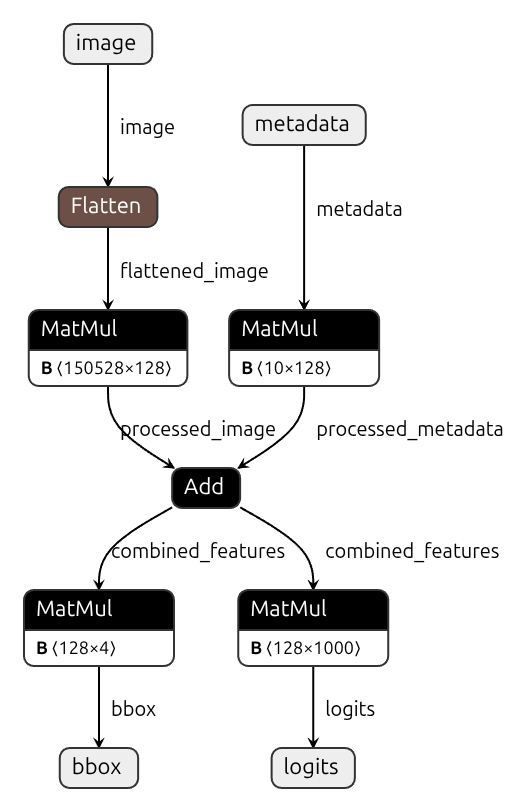
\includegraphics[height=10cm]{imgs/multi_io_net.onnx.png}
    \caption{A network with multiple inputs/outputs, mapped by declaration order.}
    \label{fig:multi-inputs-outputs}
\end{figure}


\paragraph{Hidden Node Declarations}
\label{sec:hidden-node-declarations}
In some verification applications is necessary to reason about the result of intermediate computation results at hidden nodes within the network, such as encoding features, attention mechanisms, or other internal states.
This can be achieved by declaring hidden nodes is declared using the \texttt{declare-hidden} keyword. This declaration includes a variable name for use within the \vnnlib{} specification, 
its element type, its tensor shape, and crucially, a string identifier that specifies the corresponding node name in the ONNX graph.  Multiple
hidden nodes can be trivially declared within a single network declaration. Example~\ref{lst:hidden_node} shows a \vnnlib{} network declaration with a hidden node.

\begin{figure}[h!]
    \begin{minipage}[c]{0.65\textwidth}
        \begin{lstlisting}[style=lbnf]   
(declare-network encoder
    (declare-input X Real [1,28,28])
    (declare-hidden Z Real [1,128] "encoder_output")
    (declare-output Y Real [1,10])
)\end{lstlisting}
    \end{minipage}%
    \begin{minipage}[c]{0.35\textwidth}
        \centering
        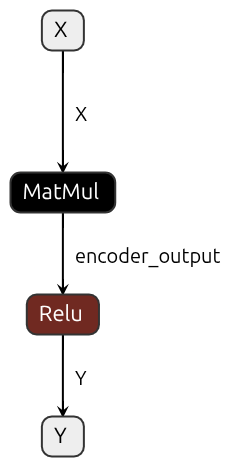
\includegraphics[height=6cm]{imgs/encoder_net.onnx.png}
    \end{minipage}
    \caption{\vnnlib{} network declaration that declares a hidden node}
    \label{fig:hidden-node}
\end{figure}

\subsubsection*{Multiple networks}
\label{sec:multi-network-declarations}
\vnnlib{} supports defining multiple networks in a single file by including multiple `(declare-network ...)` expressions. This is essential for properties that compare networks, 
such as checking for equivalence between two models or verifying properties of a composite system, like an observer-controller architecture. Example~\ref{lst:multi_network} 
shows a snippet from a \vnnlib{} file that declares two networks, \texttt{teacher\_net} and \texttt{student\_net}.

\begin{figure}[h!]
    \begin{minipage}[c]{0.6\textwidth}
        \begin{lstlisting}[style=lbnf]
(declare-network teacher
    (declare-input tX Real [1,32])
    (declare-output tY Real [1,2])
)

(declare-network student
    (declare-input sX Real [1,32])
    (declare-output sY Real [1,2])
)\end{lstlisting}
    \end{minipage}
    \begin{minipage}[c]{0.4\textwidth}
        \centering
        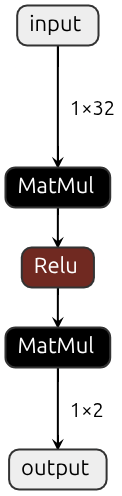
\includegraphics[height=5cm]{imgs/teacher_net.onnx.png}
        \vspace{0.5cm} 
        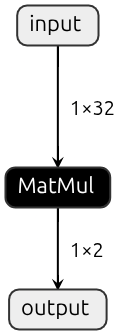
\includegraphics[height=5cm]{imgs/student_net.onnx.png}
    \end{minipage}
    \caption{Two networks declared in \vnnlib{}: \texttt{teacher\_net} and \texttt{student\_net}.}
\end{figure}


\subsection{Comments and whitespace}

Comments in \vnnlib{} are denoted by a semicolon (\texttt{;}) and extend to the end of the line. They are used for annotation, explaining logic, or providing additional context. Whitespace in \vnnlib{} is used to separate tokens and improve readability. It can include spaces, tabs, and newlines. Whitespace is ignored by the parser, except where it is necessary to separate tokens.


\section{Scoping and Typing}
\label{sec:scoping_and_typing}

\mnote{TODO: Ann Roy}

\begin{itemize}
\item Unique variable names
\item Well-scoped indices within tensor dimensions
\item Inputs/hidden/output declarations in order.
\end{itemize}


\section{Semantics}
\label{sec:semantics}

\mnote{TODO: Ann Roy}
